\documentclass[11pt,a4paper]{report}

\usepackage{xcolor}
\def\farbe{blue}

\usepackage{dclecture}

\usepackage{circuitikz}

\ctikzset{
    logic ports=ieee,
    logic ports/scale=0.8,
    logic ports/fill=lightgray
}

\usetikzlibrary{arrows,shapes.gates.logic.US,shapes.gates.logic.IEC,calc}


\usepackage{listings}
\lstset{language=Python}


\definecolor{codegreen}{rgb}{0,0.6,0}
\definecolor{codegray}{rgb}{0.9,0.9,0.9}
\definecolor{codepurple}{rgb}{0.58,0,0.82}
\definecolor{backcolour}{rgb}{0.95,0.95,0.92}

\lstdefinestyle{mystyle}{
%	morekeywords={forward,turn},
    backgroundcolor=\color{codegray},
    commentstyle=\color{codegreen},
%    keywordstyle=\color{codegreen},
    numberstyle=\tiny\color{gray},
    stringstyle=\color{codepurple},
    basicstyle=\footnotesize,
    identifierstyle=\color{blue},
    stringstyle=\color{orange},
    breakatwhitespace=false,
    breaklines=true,
    captionpos=b,
    keepspaces=true,
    numbers=left,
    numbersep=5pt,
    showspaces=false,
    showstringspaces=false,
    showtabs=false,
    tabsize=2
}

\lstset{style=mystyle}




%%% Fancy Header and Footer
\renewcommand{\headrule}{\vbox to 0pt{\hbox to\headwidth{\color{\farbe}\rule{\headwidth}{1pt}}\vss}}
\pagestyle{fancy} %eigener Seitenstil
\fancyhf{} %alle Kopf- und Fusszeilenfelder bereinigen
\fancyhead[C]{Computer Science} %Kopfzeile mitte
%\fancyhead[R]{\includegraphics[width=0.2cm]{x.png}}
\fancyfoot[C]{\thepage}


\newcommand{\bfb}[1]{{\bf \color{blue} #1}}




\begin{document}

\section*{From 1's and 0's to TikTok (or whichever App is trending today)}
A brief overview on how we can manipulate and work with very simple building blocks to create a vast global network. 
\section{The Math}
Iin this section we look at the mathematical basics of computing. 
\subsection{The 1's and the 0's}
Although some early computers were decimal machines, modern  computers are all binary. The reason for this is mainly engineering: It is relatively easy to make a switch with two positions \emph{on} and \emph{off}. Newer computers still apply this basic idea for their calculations -- just with electricity: low voltage is off (or zero) and high voltage is on (or one).

A basic storage unit of a computer is a \bfb{bit}, which is short for \bfb{binary digit}. Eight bits are called a \bfb{byte}. $1024$ bytes are a \bfb{kilobyte}, because we are dealing with powers of $2$ and $2^{10}=1024$ is closest to $1000$. The same reasoning is applied for megabytes, gigabytes, terabytes etc. 

Since one bit does not encode much information, modern computers use $64$ bits as a basic unit of storage. That means that each number, character and special symbol uses up $64$ bits of memory. This also means that a computer can not calculate with numbers that are too big -- this leads to \bfb{overflow}.

\newpage
\subsubsection{Exercises}

\begin{ex}
Convert the following binary numbers to decimal.
\begin{multicols}{4}
\begin{enumerate}
\item $10101$
\item $1110$
\item $1000001$
\item $1100110011$
\end{enumerate}
\end{multicols} 
\end{ex}
\sol{
\begin{multicols}{4}
\begin{enumerate}
\item $21$
\item $14$
\item $65$
\item $819$
\end{enumerate}
\end{multicols}
}

\begin{ex}
Convert the following decimal numbers to binary.
\begin{multicols}{4}
\begin{enumerate}
\item $42$
\item $122$
\item $2022$
\item $15$
\end{enumerate}
\end{multicols} 
\end{ex}
\sol{
\begin{multicols}{4}
\begin{enumerate}
\item $101010$
\item $1111010$
\item $11111100110$
\item $1111$
\end{enumerate}
\end{multicols}
}

\begin{ex}
How many bits are in a megabyte?
\end{ex}
\sol{$8'388'608$}

\subsection{Different Bases}
The \bfb{base} of a number system indicates which powers are represented by each position. In our standard \bfb{decimal} system each position is a power of $10$, where the first position are the $1$'s ($10^0=1)$.  In the \bfb{binary} system each position is a power of $2$; so $1$, $2$, $4$, etc.

In this way any natural number can be the base of a number system. We have already seen the \bfb{hexadecimal} system with a base of $16$, but any other number could be the base of a number system. Sometimes you may see a small subscript number indicating the base:
\[
11100_{2} = 28_{10}
\]
\[
122_{3}=17_{10}
\]
\[
122_{7} = 65_{10}
\]



\subsubsection{Exercises}
\begin{ex}
Convert the following numbers to decimal.
\begin{multicols}{4}
\begin{enumerate}
\item $111_{3}$
\item $111_{7}$
\item $1010_{4}$
\item $5_{42}$
\end{enumerate}
\end{multicols} 
\end{ex}
\sol{
\begin{multicols}{4}
\begin{enumerate}
\item $13$
\item $57$
\item $68$
\item $5$
\end{enumerate}
\end{multicols}
}

\subsection{How to Deal with Negative Numbers}
Addition with binary numbers is relatively straightforward: We just add and carry each position as with our decimal addition. For subtraction we use a simple trick: Instead of $7-2$ we write $7+(-2)$. This way if we have a technique for writing $-2$ in binary, then we can also calculate the difference. 

The technique is called \bfb{2's complement} and works as follows: 
\begin{enumerate}
\item[1.] Find the positive binary value for the negative number you want to represent. Write out any leading zeros.
\item[2.] Invert or find the complement of each bit in the number.
\item[3.] Add 1 to this number. 
\end{enumerate}

For this to work each number has to have a fixed

{\bf Example.}  In a computer system with a four bit storage system
\[
1 = 0001_2 \qaq -1 = 1111_2
\]
\[
4 = 0100 \qaq -4 = 1100_2
\]



\subsubsection{Exercises}

\begin{ex}
Use 2's complement to calculate $7-5$ in binary. Use a 4 bit notation.
\end{ex}

\begin{ex}
Use 2's complement to calculate $5-5$ in binary. Use a 4 bit notation.
\end{ex}



\subsection{How to Deal with Fractions}
In computing any numbers that are not \bfb{integers} are called \bfb{real}. Since there are only a finite number of storage spaces on a computer there is also only finite precision. The way a computer represents a fraction is by placing a point somewhere in the number. Now the digits to the left signify integers and digits to the right are fractional powers of $2$:
\[
11.11_2 = 3.75
\]


\subsubsection{Exercises}
\begin{ex}
Convert $0.5$ into binary.
\end{ex}
\sol{$0.1_2$}


\begin{ex}
Convert $\dfrac{1}{64}$ into binary.
\end{ex}
\sol{$0.000001_2$}


\begin{ex}
Convert $\dfrac{1}{3}$ into binary.
\end{ex}
\sol{$0.\overline{01}_2$}


\begin{ex}
Convert $0.2$ into binary.
\end{ex}
\sol{$0.\overline{0011}_2$}

\newpage

\subsubsection{Solutions}
\printcursols

\newpage
\section{Data Representation}

We saw in the previous section how numbers are represented and manipulated by computers. To have a fully functional modern computer we need many other types of data: text, images, sound etc. 

In this section we will regard the basics of these data representations. We have seen many of these ideas before. 

\subsection{Representing Text}

ASCII stands for American Standard Code for Information Interchange. It is a character encoding standard used for representing text and certain special characters in computers. 

Below is the complete 7 bit ASCII character table and decimal equivalent.

\centfig{0.9}{ASCII.png}
\hfill source: {\url{https://en.m.wikipedia.org/wiki/File:ASCII-Table.svg}}

The 7 bit ASCII table is no longer really viable, since we need many more symbols in modern computers. For a while there was an extended ASCII table with 8 bits. However, modern encoding uses the Unicode format which is backwards compatible with ASCII but allows for many, many more different characters.

For an explanation on how Unicode works, please watch the following video: \url{https://youtu.be/MijmeoH9LT4}

\subsection{Representing Audio}

Computer audio is encoded by taking the waveforms of an audio input and transcoding that into a digital representation. 

A sound wave, in red, represented digitally, in blue (after sampling and 4-bit quantization):
\centfig{0.8}{audio}
\hfill \emph{source: \url{https://www.wikiwand.com/en/Digital_audio}}

\subsection{Representing Images}

Data in computers is stored and transmitted as a series of ones and zeros (also known as Binary). 

To store an image on a computer, the image is broken down into tiny elements called pixels. A \bfb{pixel} (short for picture element) represents one colour. The number of pixels in an image is called its \bfb{resolution}. An image with a resolution of 1024 by 798 pixels has 1024 x 798 pixels (817,152 pixels). 

For a monochrome image each pixel can be represented by one bit. For webpages and most standard applications we use a 16 bit colorspace. In  certain special situations, we may want more colors and perhaps an \bfb{alpha channel}. The alpha channel can encode transparency and other shading information.

\subsection{Representing Video}

Video information is one of the most complex types of information saved on a computer. It contains the equivalent of thousands of images and audio. 

\newpage

\section{Gates and Circuits}

Computers are electronic devices - they take electrical power, translate it into ones and zeros and then manipulate those digits to give us any number of outputs: images, text files, videos, webpages etc. 

They do this using \bfb{gates} and \bfb{circuits}. A gate is an electronic device that takes one or more input signals (current) and produces a single output. A circuit is a combination of gates that can fulfil a task (e.g. adding, storing data, retrieving data etc.).

\subsection{Gates}

Gates are also  sometimes called \bfb{logic gates} because they perform a single logic operation. We will look at the basic gates and some notation. There are three different ways in which these gates and their logic are represented; all have their advantages and disadvantages. 


\bfb{Logic diagrams} are graphical representations of logic gates and their connections; these are used to show how complex circuits are created from simple pieces. The individual gates have standardized symbols.

\bfb{Truth tables} write out all possiible inputs and outputs and are useful for determining the output of a circuit for a given input.

\bfb{Boolean Algebra} is a purely algebraic notation for logic and is mainly used for theoretical proofs and calculations. 

\newpage
\subsubsection{The {\bf NOT} Gate}
The not gate takes an input and reverses it. $1$ turns to $0$, TRUE to FALSE, Black to White etc. In technical terms it changes the current from a high voltage to a low voltage. The mathematical symbol for NOT is $\neg$.

\renewcommand{\arraystretch}{1.5}
\begin{center}
\begin{tabular}{c|c|c}
Logic diagram & Truth table & Algebra \\
\hline
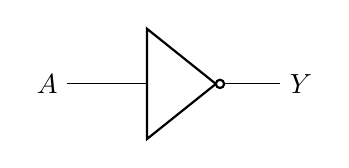
\begin{tikzpicture}[baseline=1]
\node[not port, draw] at ($(1,0)$) (Not) {};
\draw ++(-0.5,0) node[left](A){$A$} -- (Not.in);
\draw (Not.out) -- ++(0.5,0) node[right](){$Y$};
\end{tikzpicture}
& 
\renewcommand{\arraystretch}{1}
\begin{tabular}{c|c}
$A$ & $Y$ \\
\hline
$0$ & $1$ \\
$1$ & $0$
\end{tabular}
& $Y=\neg A$
\end{tabular}
\end{center}


\subsubsection{The AND Gate}
The AND gate returns a $1$ if and only if both inputs $A$ {\bf and} $B$ are $1$.
\begin{center}
\begin{tabular}{c|c|c}
Logic diagram & Truth table & Algebra \\
\hline
\begin{tikzpicture}[baseline=1]
\node[and port] at ($(1,0)$) (a) {};
\draw ++(-0.5,0.25) node[left](A){$A$} -- (a.in 1);
\draw ++(-0.5,-0.25) node[left](B){$B$} -- (a.in 2);
\draw (Not.out) -- ++(0.5,0) node[right](){$Y$};
\end{tikzpicture}
& 
\renewcommand{\arraystretch}{1}
\begin{tabular}{c|c|c}
$A$ & $B$ & $Y$ \\
\hline
$0$ & $0$ & $0$\\
$1$ & $0$ & $0$\\
$0$ & $1$ & $0$\\
$1$ & $1$ & $1$
\end{tabular}
& $Y= A\wedge B$
\end{tabular}
\end{center}

\subsubsection{The OR Gate}
The OR gate returns a $1$ if one of inputs $A$ {\bf or} $B$ are $1$.
\begin{center}
\begin{tabular}{c|c|c}
Logic diagram & Truth table & Algebra \\
\hline
\begin{tikzpicture}[baseline=1]
\node[or port] at ($(1,0)$) (a) {};
\draw ++(-0.5,0.25) node[left](A){$A$} -- (a.in 1);
\draw ++(-0.5,-0.25) node[left](B){$B$} -- (a.in 2);
\draw (Not.out) -- ++(0.5,0) node[right](){$Y$};
\end{tikzpicture}
& 
\renewcommand{\arraystretch}{1}
\begin{tabular}{c|c|c}
$A$ & $B$ & $Y$ \\
\hline
$0$ & $0$ & $0$\\
$1$ & $0$ & $1$\\
$0$ & $1$ & $1$\\
$1$ & $1$ & $1$
\end{tabular}
& $Y= A\lor B$
\end{tabular}
\end{center}

\subsubsection{The XOR Gate}
The XOR gate returns a $1$ if one of inputs $A$ {\bf or} $B$ are $1$ but not both.
\begin{center}
\begin{tabular}{c|c|c}
Logic diagram & Truth table & Algebra \\
\hline
\begin{tikzpicture}[baseline=1]
\node[xor port] at ($(1,0)$) (a) {};
\draw ++(-0.5,0.25) node[left](A){$A$} -- (a.in 1);
\draw ++(-0.5,-0.25) node[left](B){$B$} -- (a.in 2);
\draw (Not.out) -- ++(0.5,0) node[right](){$Y$};
\end{tikzpicture}
& 
\renewcommand{\arraystretch}{1}
\begin{tabular}{c|c|c}
$A$ & $B$ & $Y$ \\
\hline
$0$ & $0$ & $0$\\
$1$ & $0$ & $1$\\
$0$ & $1$ & $1$\\
$1$ & $1$ & $0$
\end{tabular}
& $Y= A\oplus B$
\end{tabular}
\end{center}

\subsubsection{NAND and NOR Gates}
NAND and NOR gates are the inverses of AND and OR gates respectively. 

\begin{center}
\begin{tabular}{c|c|c}
Logic diagram & Truth table & Algebra \\
\hline
\begin{tikzpicture}[baseline=1]
\node[nand port] at ($(1,0)$) (a) {};
\draw ++(-0.5,0.25) node[left](A){$A$} -- (a.in 1);
\draw ++(-0.5,-0.25) node[left](B){$B$} -- (a.in 2);
\draw (Not.out) -- ++(0.5,0) node[right](){$Y$};
\end{tikzpicture}
& 
\renewcommand{\arraystretch}{1}
\begin{tabular}{c|c|c}
$A$ & $B$ & $Y$ \\
\hline
$0$ & $0$ & $1$\\
$1$ & $0$ & $1$\\
$0$ & $1$ & $1$\\
$1$ & $1$ & $0$
\end{tabular}
& $Y= \neg(A\wedge B)$ \\
\hline
\begin{tikzpicture}[baseline=1]
\node[nor port] at ($(1,0)$) (a) {};
\draw ++(-0.5,0.25) node[left](A){$A$} -- (a.in 1);
\draw ++(-0.5,-0.25) node[left](B){$B$} -- (a.in 2);
\draw (Not.out) -- ++(0.5,0) node[right](){$Y$};
\end{tikzpicture}
& 
\renewcommand{\arraystretch}{1}
\begin{tabular}{c|c|c}
$A$ & $B$ & $Y$ \\
\hline
$0$ & $0$ & $1$\\
$1$ & $0$ & $0$\\
$0$ & $1$ & $0$\\
$1$ & $1$ & $0$
\end{tabular}
& $Y= \neg(A\lor B)$
\end{tabular}
\end{center}



\end{document}
